\documentclass[10pt,a4paper]{article}
\usepackage[utf8]{inputenc}
\usepackage{amsmath}
\usepackage{amsfonts}
\usepackage{amssymb}
\usepackage{graphicx}
\usepackage[left=2cm,right=2cm,top=2cm,bottom=2cm]{geometry}
\author{Rasmus Kristoffer Pedersen}
\begin{document}

\section{Model description}
\subsection{Model assumptions}
The considered model is based on the classic SIR-model, extended to consider two seperate strains of diseases.
The model does not consider cross-immunity, however, simultanious infections is omitted. 
Furthermore, vaccination toward one of the two strains is considered. 

With $I$ denoting one strain and $Y$ denoting the other, the following variables are considered:
\begin{itemize} 
    \item $S$: Unvaccinated, susceptible to both strains.
    \item $V$: Vaccinated. Immune to strain $Y$ but susceptible to strain $I$.
    \item $I_S$: Unvaccinated infected with strain $I$.
    \item $I_V$: Vaccinated infected with strain $I$.
    \item $I_{0,1}$: Recovered from strain $Y$, infected with strain $I$.
    \item $Y$: Infected with strain $Y$. 
    \item $Y_{1,0}$: Recovered from strain $I$, infected with strain $Y$.
    \item $R_{0,1}$: Recovered from strain $Y$, susceptible to strain $I$.
    \item $R_{1,0}$: Recovered from strain $I$, susceptible to strain $Y$.
    \item $R_{1,1}$: Recovered from both strains, or recovered from strain $I$ and vaccinated.
\end{itemize}

\subsection{``Reactions''}
\begin{align}
    S & \Rightarrow I_S & \text{Infected with strain }I \\ 
    V & \Rightarrow I_V & \text{Infected with strain }I \\ 
    S & \Rightarrow Y & \text{Infected with strain }Y \\ 
    I_S & \Rightarrow R_{0,1} & \text{Recovery from infection} \\ 
    I_V & \Rightarrow R_{1,1} & \text{Recovery from infection} \\ 
    Y & \Rightarrow R_{1,0} & \text{Recovery from infection} \\ 
    R_{0,1} & \Rightarrow I_{0,1} & \text{Infected with strain }I \\ 
    R_{1,0} & \Rightarrow Y_{1,0} & \text{Infected with strain }Y \\ 
    I_{0,1} & \Rightarrow R_{1,1} & \text{Recovery from infection} \\ 
    Y_{1,0} & \Rightarrow R_{1,1} & \text{Recovery from infection} \\ 
\end{align}

\subsection{Equations}


% dS   = - (beta_IS_S * IS + beta_IV_S * IV + beta_I01_S * I01 + beta_Y_S * Y + beta_Y10_S * Y10) * S
% dV   = - (beta_IS_V * IS + beta_IV_V * IV + beta_I01_V * I01) * V
% dIS  =   (beta_IS_S * IS + beta_IV_S * IV + beta_I01_S * I01) * S               - gamma_IS * IS 
% dIV  =   (beta_IS_V * IS + beta_IV_V * IV + beta_I01_V * I01) * V               - gamma_IV * IV
% dY   =   (beta_Y_S * Y + beta_Y10_S * Y10) * S                                  - gamma_Y * Y 
% dR01 = - (beta_IS_R01 * IS + beta_IV_R01 * IV + beta_I01_R01 * I01) * R01       + gamma_Y  * Y  
% dR10 = - (beta_Y_R10 * Y + beta_Y10_R10 * Y10) * R10                            + gamma_IS * IS
% dI01 =   (beta_IS_R01 * IS + beta_IV_R01 * IV + beta_I01_R01 * I01) * R01       - gamma_I01 * I01 
% dY10 =   (beta_Y_R10 * Y + beta_Y10_R10 * Y10) * R10   

\begin{align}
    \dot{S} &= - \left(\beta_{I_S,S} I_S + \beta_{I_{V},S} I_V  + \beta_{I_{0,1},S} I_{0,1} + \beta_{Y,S} Y + \beta_{Y_{10},S} Y_{10}\right) S \\
    \dot{V} &= - \left(\beta_{I_S,V} I_S + \beta_{I_{V},V} I_V  + \beta_{I_{0,1},V} I_{0,1} \right) V \\ 
    \dot{I_S} &= \left(\beta_{I_S,S} I_S + \beta_{I_{V},S} I_V  + \beta_{I_{0,1},S} I_{0,1} \right) S - \gamma_{I_S} I_S \\
    \dot{I_V} &= \left(\beta_{I_S,V} I_S + \beta_{I_{V},V} I_V  + \beta_{I_{0,1},V} I_{0,1} \right) V - \gamma_{I_V} I_V \\
    \dot{Y} &= \left(\beta_{Y,S} Y + \beta_{Y_{1,0},S} Y_{1,0}\right) S - \gamma_{Y} Y \\
    \dot{R_{0,1}} &= - \left(\beta_{I_S,R_{0,1}} I_S + \beta_{I_{V},R_{0,1}} I_V  + \beta_{I_{0,1},R_{0,1}} I_{01} \right) R_{0,1} + \gamma_{Y} Y \\ 
    \dot{R_{1,0}} &= - \left(\beta_{Y,R_{1,0}} Y + \beta_{Y_{1,0},R_{1,0}} Y_{1,0}\right) R_{1,0} + \gamma_{I_S} I_S \\
    \dot{I_{0,1}} &=   \left(\beta_{I_S,R_{0,1}} I_S + \beta_{I_{V},R_{0,1}} I_V  + \beta_{I_{0,1},R_{0,1}} I_{01} \right) R_{0,1} - \gamma_{I_{0,1}} I_{0,1} \\ 
    \dot{Y_{1,0}} &=   \left(\beta_{Y,R_{1,0}} Y + \beta_{Y_{1,0},R_{1,0}} Y_{1,0}\right) R_{1,0} - \gamma_{Y_{1,0}} Y_{1,0} \\
    \dot{R_{1,1}} &= \gamma_{I_V} I_V + \gamma_{I_{0,1}} I_{0,1} + \gamma_{Y_{1,0}} Y_{1,0}
\end{align}
As the equations sum to zero, one equation can be omitted. Hence, we define 
\begin{equation}
R_{1,1} = 1 - S - V - I_S - I_V - I_{0,1} - Y - Y_{1,0} - R_{0,1} - R_{1,0}
\end{equation}

\subsection{Simplifying assumptions}
We now assume that transmission rates $\beta_{a,b}$ are the product of a infectivity rate, $\alpha_a$ and a susceptivity rate, $\mu_b$, i.e. $\beta_{a,b} = \alpha_a \mu_b$. 
This allows for a simplifcation of the system of differential equations:

\begin{align}
    \dot{S} &= - \mu_S (I_T + Y_T) S \\ 
    \dot{V} &= - \mu_V I_T V \\ 
    \dot{I_S} &= \mu_S I_T S - \gamma_{I_S} \\ 
    \dot{I_V} &= \mu_V I_T V - \gamma_{I_V} I_V \\
    \dot{Y} &= \mu_S Y_T S - \gamma_{Y} Y \\
    \dot{R_{0,1}} &= - \mu_{R_{0,1}} I_T R_{0,1} + \gamma_{Y} Y \\ 
    \dot{R_{1,0}} &= - \mu_{R_{1,0}} Y_T R_{1,0} + \gamma_{I_S} I_S \\
    \dot{I_{0,1}} &=   \mu_{R_{0,1}} I_T R_{0,1} - \gamma_{I_{0,1}} I_{0,1} \\ 
    \dot{Y_{1,0}} &=   \mu_{R_{1,0}} Y_T R_{1,0} - \gamma_{Y_{1,0}} Y_{1,0} 
\end{align}
where $I_T$ and $Y_T$ denote the infectious pressure of strain $I$ and $Y$ respectively, defined as:
\begin{align}
    I_T &= \alpha_{I_S} I_S + \alpha_{I_V} I_V + \alpha_{I_{0,1}} I_{0,1} \\ 
    Y_T &= \alpha_{Y} Y + \alpha_{Y_{1,0}} Y_{1,0} 
\end{align}

A further assumption that infectivity is independent of the disease history of an individual could suggest a further simplification:
With $\alpha_I = \alpha_{I_S} = \alpha_{I_V} = \alpha_{I_{0,1}}$ and $\alpha_Y = \alpha_{Y_{1,0}}$ we can write:
\begin{align}
    I_T &= \alpha_I \left(I_S + I_V + I_{0,1} \right)\\ 
    Y_T &= \alpha_{Y} \left(Y + Y_{1,0} \right)
\end{align}

\section{Model simulations}
In the following simulations, all recovery parameters are equal, $\gamma = \frac{1}{7}$ and all transmission parameters are equal, $\beta= \frac{2}{7}$.
\subsection{Single strain epidemics}
\begin{figure}[ht]\centering
    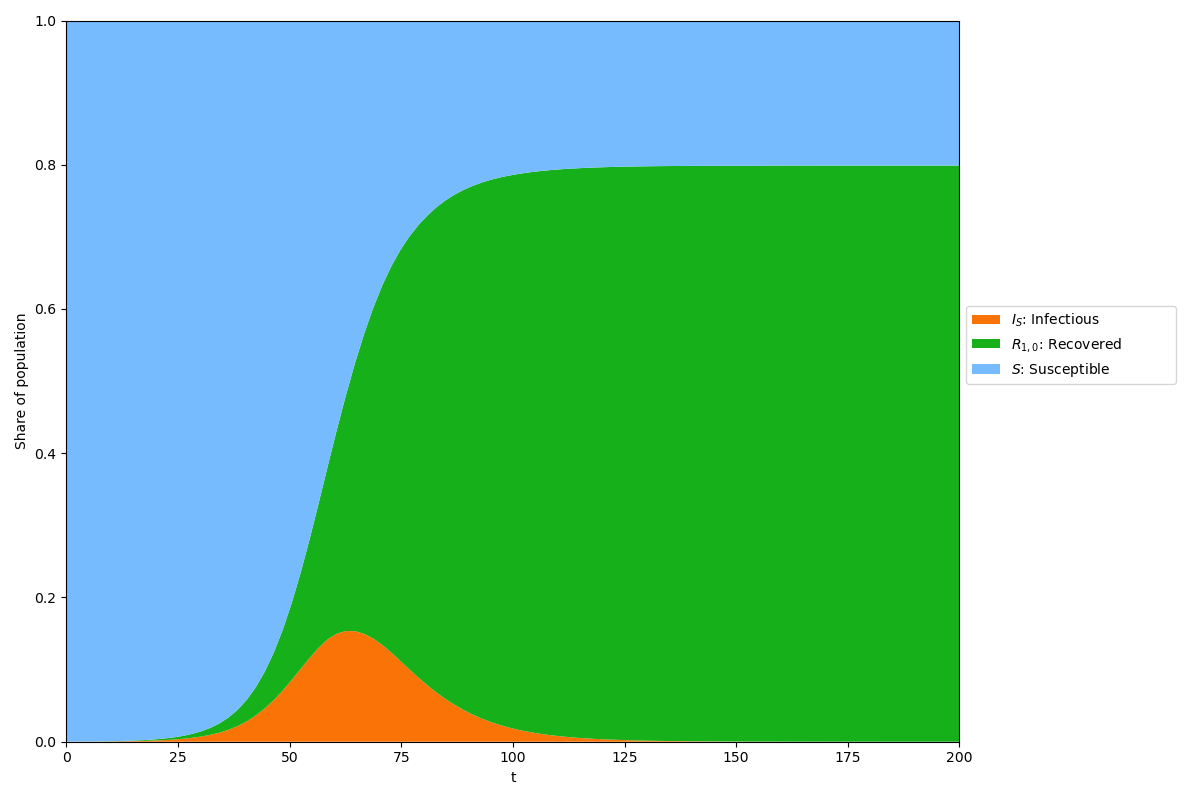
\includegraphics[width=0.9\linewidth]{../Figures/TwoStrainModel_OnlyI.png}
    \caption{Single epidemic with strain $Y$. $I_S(0)=0.0001$ and $S(0)=1-0.0001$}
\end{figure}
\begin{figure}[ht]\centering
    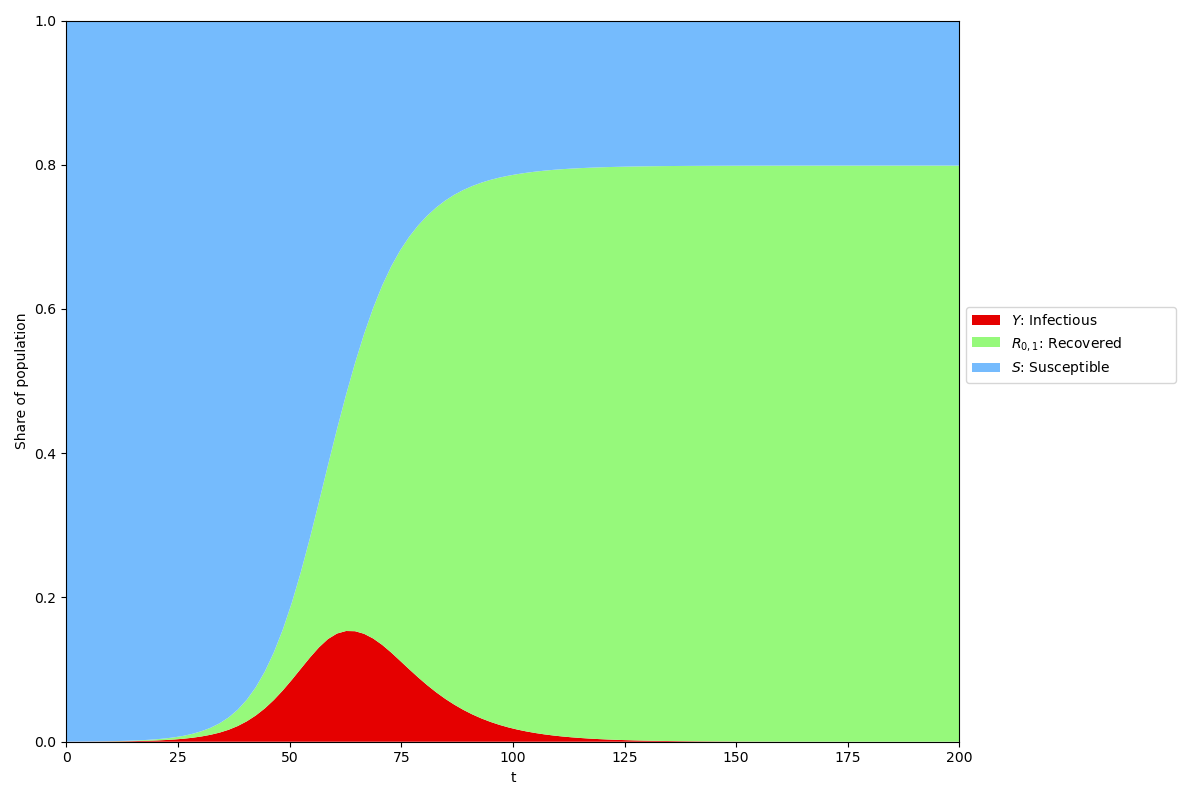
\includegraphics[width=0.9\linewidth]{../Figures/TwoStrainModel_OnlyY.png}
    \caption{Single epidemic with strain $Y$. $Y(0)=0.0001$ and $S(0)=1-0.0001$}
\end{figure}
 

\subsection{Single strain epidemics, with vaccination}
\begin{figure}[ht]\centering
    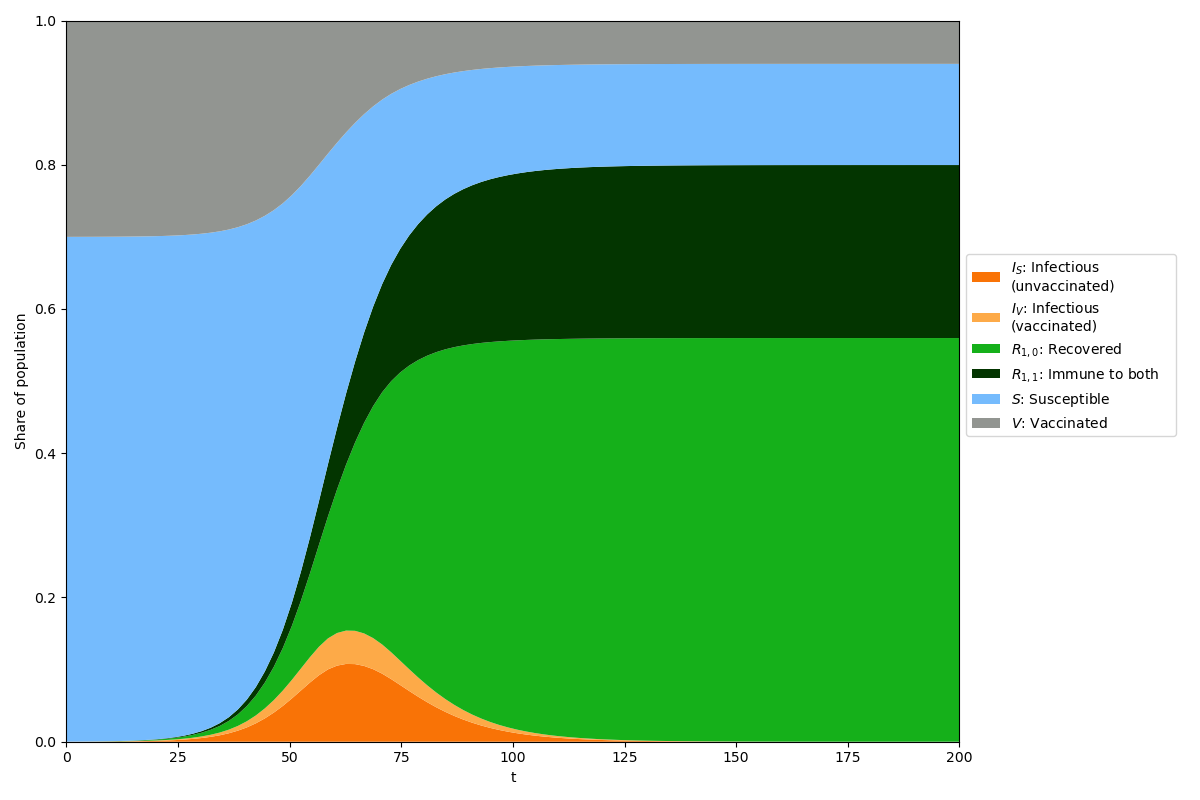
\includegraphics[width=0.9\linewidth]{../Figures/TwoStrainModel_OnlyI_Vacc.png}
    \caption{Single epidemic with strain $Y$. $I_S(0)=0.0001$, $V(0)=0.4$ and $S(0)=1-0.4-0.0001=0.5999$}
\end{figure}
\begin{figure}[ht]\centering
    \includegraphics[width=0.9\linewidth]{../Figures/TwoStrainModel_OnlyY_Vacc.png}
    \caption{Single epidemic with strain $Y$. $Y(0)=0.0001$, $V(0)=0.4$ and $S(0)=1-0.4-0.0001=0.5999$}
\end{figure}


\subsection{Subsequent epidemics}


\begin{figure}[ht]\centering
    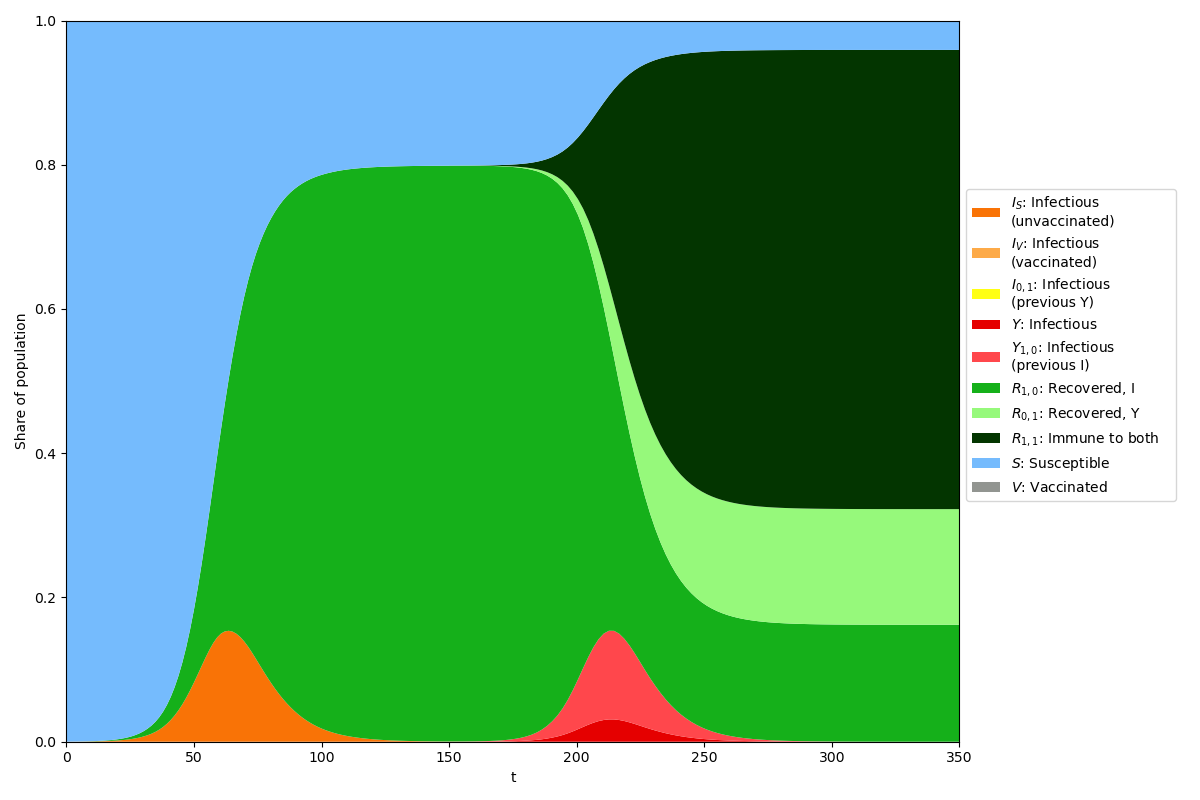
\includegraphics[width=0.9\linewidth]{../Figures/TwoStrainModel_IthenY.png}
    \caption{Subsequent epidemics, strain $I$ then $Y$. $I_S(0)=0.0001$ and $S(0)=0.9999$. At time $t=150$, $0.0001$ is subtracted from $S$ and added to $Y$.}
\end{figure}
\begin{figure}[ht]\centering
    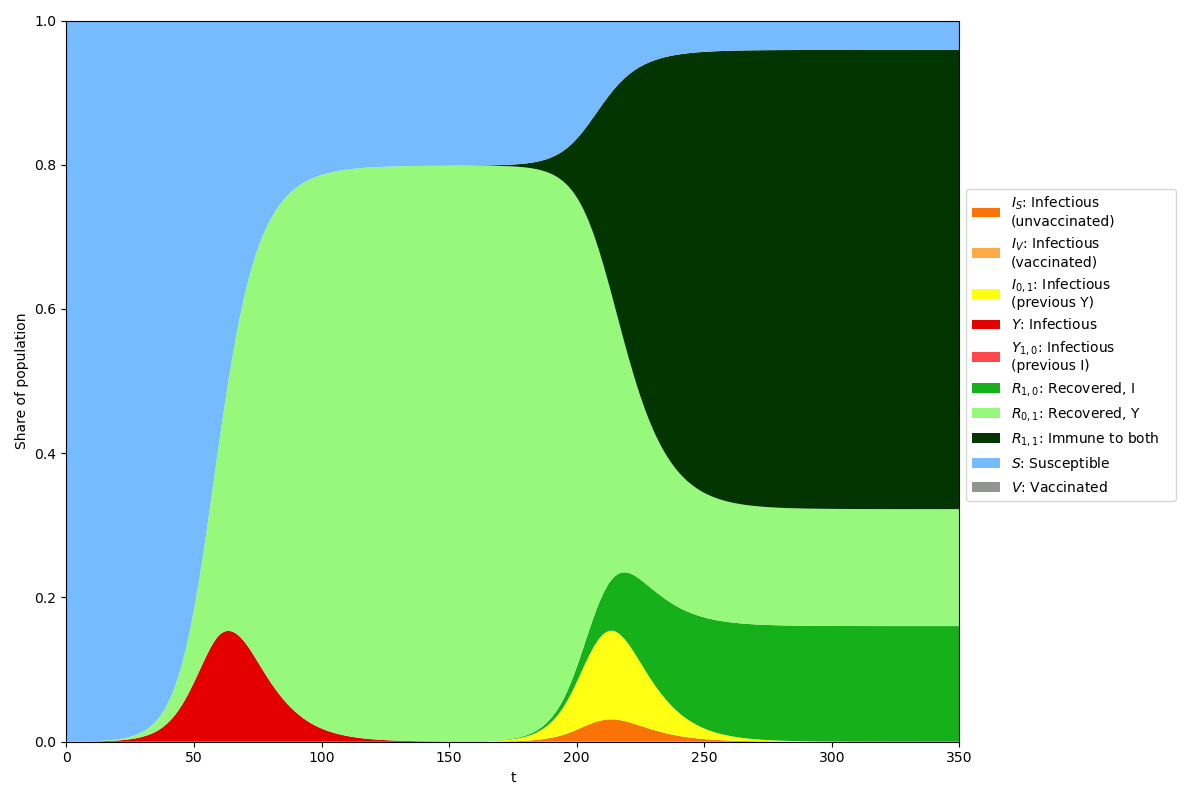
\includegraphics[width=0.9\linewidth]{../Figures/TwoStrainModel_YthenI.png}
    \caption{Subsequent epidemics, strain $Y$ then $I$. $Y(0)=0.0001$ and $S(0)=0.9999$. At time $t=150$, $0.0001$ is subtracted from $S$ and added to $I$.}
\end{figure}



\begin{figure}[ht]\centering
    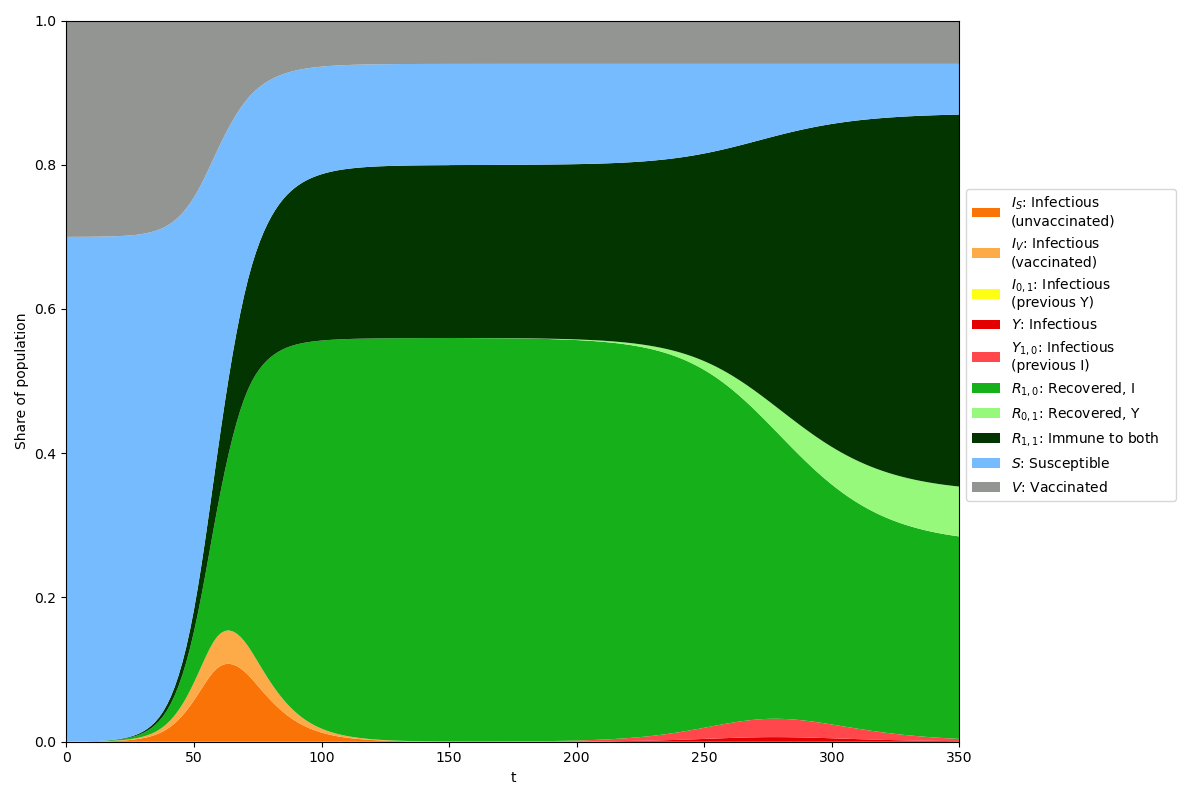
\includegraphics[width=0.9\linewidth]{../Figures/TwoStrainModel_IthenY_Vacc.png}
    \caption{Subsequent epidemics, strain $I$ then $Y$. $I_S(0)=0.0001$, $V(0)=0.4$ and $S(0)=0.5999$. At time $t=150$, $0.0001$ is subtracted from $S$ and added to $Y$.}
\end{figure}
\begin{figure}[ht]\centering
    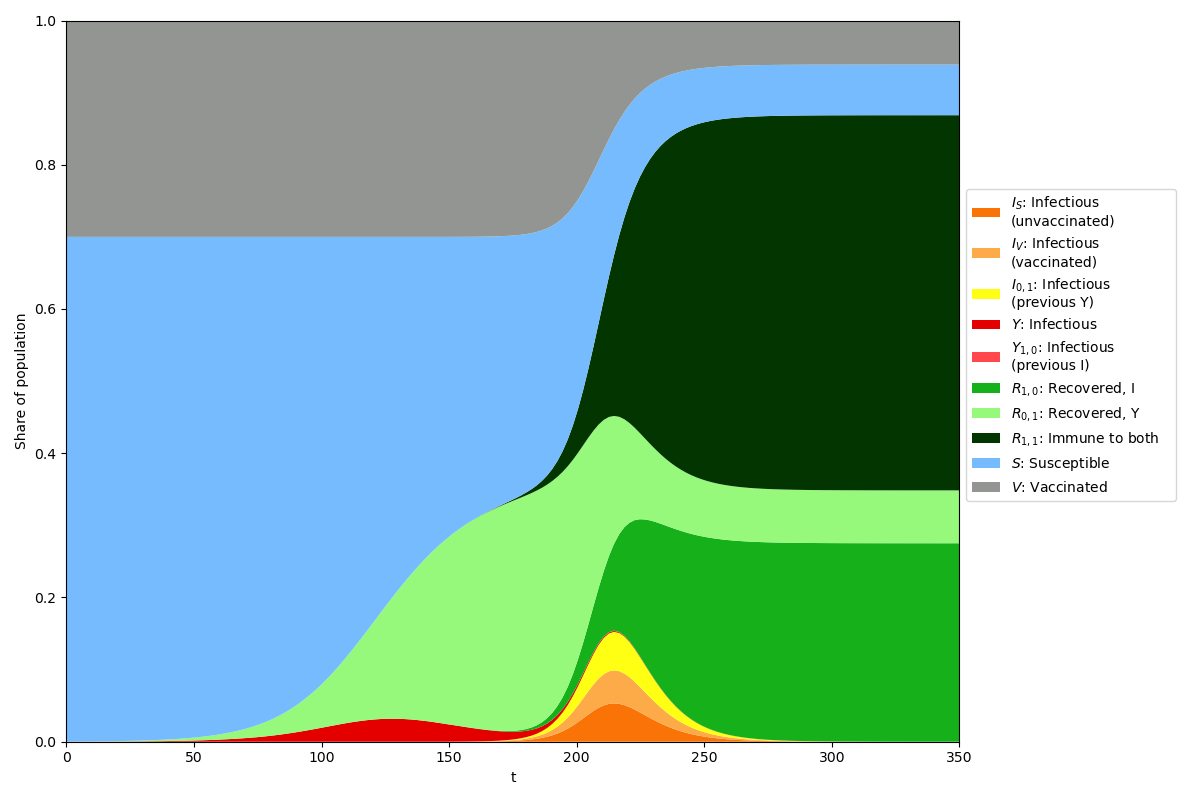
\includegraphics[width=0.9\linewidth]{../Figures/TwoStrainModel_YthenI_Vacc.png}
    \caption{Subsequent epidemics, strain $Y$ then $I$. $Y(0)=0.0001$, $V(0)=0.4$ and $S(0)=0.5999$. At time $t=150$, $0.0001$ is subtracted from $S$ and added to $I$.}
\end{figure}


\end{document}